% FytcNote-2024-1-part (c) by Quan-feng WU <wuquanfeng@ihep.ac.cn>
% 
% FytcNote-2024-1-part is licensed under a
% Creative Commons Attribution-NonCommercial-NoDerivatives 4.0 International License.
% 
% You should have received a copy of the license along with this
% work. If not, see <https://creativecommons.org/licenses/by-nc-nd/4.0/>.

\documentclass{article}

\usepackage{amssymb}
\usepackage{authblk}
\usepackage[sorting=none, style=numeric-comp]{biblatex}
    \addbibresource{references.bib}
\usepackage[compat=1.1.0]{tikz-feynhand}
\usepackage[a4paper, margin=2.5cm]{geometry}
\usepackage[colorlinks=true]{hyperref}
\usepackage{pgfplots}
    \pgfplotsset{compat=1.18}
\usepackage{physics}
\usepackage{slashed}
\usepackage{subcaption}
\usepackage{tensor}

% FytcNote-2024-1-part (c) by Quan-feng WU <wuquanfeng@ihep.ac.cn>
% 
% FytcNote-2024-1-part is licensed under a
% Creative Commons Attribution-NonCommercial-NoDerivatives 4.0 International License.
% 
% You should have received a copy of the license along with this
% work. If not, see <https://creativecommons.org/licenses/by-nc-nd/4.0/>.

\newcommand{\email}[1]{\footnote{E-mail: \href{mailto:#1}{#1}}}
\newcommand{\eg}{\textit{e.g.}}
\newcommand{\ie}{\textit{i.e.}}
\newcommand{\license}{\footnote{This note © 2024 by \href{https://github.com/Fenyutanchan}{Quan-feng WU} is licensed under \href{https://creativecommons.org/licenses/by-nc-/4.0/}{CC BY-NC-ND 4.0}. \faCreativeCommons \faCreativeCommonsBy \faCreativeCommonsNc \faCreativeCommonsNd}}

% FytcNote-2024-1-part (c) by Quan-feng WU <wuquanfeng@ihep.ac.cn>
% 
% FytcNote-2024-1-part is licensed under a
% Creative Commons Attribution-NonCommercial-NoDerivatives 4.0 International License.
% 
% You should have received a copy of the license along with this
% work. If not, see <https://creativecommons.org/licenses/by-nc-nd/4.0/>.

\DeclareMathOperator{\diag}{diag}
\newcommand{\MP}{M_\mathrm{P}}
\newcommand{\const}{\mathrm{const.}}
\newcommand{\ee}{\mathrm{e}}
\newcommand{\ii}{\mathrm{i}}


\title{Part of Calculation Note for Abundance Evolution of Scalar Boson}
\author[a]{Quan-feng WU\email{wuquanfeng@ihep.ac.cn}}
\affil[a]{Institute of High Energy Physics, Chinese Academy of Sciences, Beijing 100049, China}
\affil[b]{University of Chinese Academy of Sciences, Beijing 100049, China}
\date{[FytcNote-2024-1-part] Version 1.0.0 built on May 30, 2024}

\begin{document}
    \maketitle

    \begin{abstract}
        This is a part of the calculation note for problem \#4 in Prof.~Dr.~Xu Xun-Jie's Coffee Medal, which is available at \url{https://xunjiexu.github.io/files/questions-v2.pdf}.
        In this problem, a 100 MeV hypothetical scalar boson only coupled to the electron is considered, where the Yukawa coupling is given by $y = 10^{-12}$.
        The initial abundance of the scalar boson in the early universe is zero at a sufficiently high temperature.
        In this part note, I will only show a the calculations for the collision term and some useful integrals.
    \end{abstract}

    \tableofcontents
    \newpage

    \section{Problem Statement}
        This is problem \#4 in Prof.~Dr.~Xu Xun-Jie's Coffee Medal, which is available at \url{https://xunjiexu.github.io/files/questions-v2.pdf}.
        The problem statement is as follows:

        \paragraph{Calculations in cosmology II:}
        Consider a 100 MeV hypothetical scalar boson only coupled to the electron, with the Yukawa coupling $y = 10^{-12}$. Assuming its initial abundance in the early universe at a sufficiently high temperature is zero, compute its subsequent cosmological evolution.

    \section{Problem Analysis}
        First, we denote the scalar boson as $\phi$.
        To compute the subsequent cosmological evolution of the scalar boson, the Boltzmann equation for flat universe is required, which is given by \cite{Dodelson:2020MC}
        \begin{equation}
            \dv{n_\phi(t)}{t} + 3 H n_\phi(t) = \int \frac{\dd[3]{\vb{p}_\phi}}{\qty(2 \pi)^3 2 E_\phi} C[f_\phi],
            \label{eq:Boltzmann-equation}
        \end{equation}
        where $n_\phi(t)$ is the number density of the scalar boson $\phi$, $H := \dot{a} / a$ is the Hubble parameter, and $C[f_\phi]$ is the collision term with the distribution function $f_\phi(\vb{x}; \vb{p}; t)$ for the scalar boson $\phi$.
        The collision term $C[f_\phi]$ is the sum of all possible processes that can change the number density of the scalar boson $\phi$, i.e.,
        \begin{equation}
            C[f_\phi] = \sum_p C_p[f_\phi]
        \end{equation}
        with $C_p[f_\phi]$ being the collision term for the process $p$.

        Generally, we can consider the $\phi + \qty{n} \leftrightarrow \qty{m}$ process, which means that $n + 1$ particles (including the target particle $\phi$) and $m$ particles are converting to each other.
        Therefore, the collision term for the process $\phi + \qty{n} \leftrightarrow \qty{m}$ can be written as \cite{Dodelson:2020MC}
        \begin{equation}
            \begin{aligned}
                C_{\phi + \qty{n} \leftrightarrow \qty{m}}[f_\phi] = \int \qty(\prod_{i=1}^n \frac{\dd[3]{\vb{p}_i}}{\qty(2 \pi)^3 2 E_i}) \qty(\prod_{j=1}^m \frac{\dd[3]{\vb{q}_j}}{\qty(2 \pi)^3 2 E_j}) \qty(2 \pi)^4 \delta^{(4)}\qty(p_\phi + \sum_{i=1}^n p_i - \sum_{j=1}^m q_j) \\
                {} \times \qty{ \begin{aligned}
                    \frac{1 + f_\phi(\vb{p}_\phi)}{S} \qty[\prod_{j=1}^m f_j(\vb{q}_j)] \qty(\prod_{i=1}^n \qty[1 + s_i f_i(\vb{p}_i)]) \overline{\sum} \abs{\mathcal{M}_{\phi + \qty{n} \leftarrow \qty{m}}}^2 \\
                    - \frac{f_\phi(\vb{p}_\phi)}{S} \qty[\prod_{i=1}^n f_i(\vb{p}_i)] \qty(\prod_{j=1}^m \qty[1 + s_j f_j(\vb{q}_j)]) \overline{\sum} \abs{\mathcal{M}_{\phi + \qty{n} \to \qty{m}}}^2
                \end{aligned} },
            \end{aligned}
            \label{eq:collision-term}
        \end{equation}
        where $S$ are the identical particle factors\footnote{
            We can, for example, consider the process of $n_\mathrm{t} p_\mathrm{t} + n_1 p_1 + n_2 p_2 + \cdots n_\ell p_\ell \leftrightarrow m_\mathrm{t} p_\mathrm{t} + m_1 q_1 + m_2 q_2 + \cdots m_k q_k$, where $n_i$ and $m_j$ are the number of particles and $p_i$ and $q_j$ are the different species of particles in each side of the process, respectively.
            Notice that the target particle is denote with the subscript ``t".
            Then the identical particle factor are given by $S = \abs{n_\mathrm{t} - 1}! n_1! n_2! \cdots n_\ell! \abs{m_\mathrm{t} - 1}! m_1! m_2! \cdots m_k!$, where the convention $0! = 1$ is used.
            The reason for the factors of $\abs{n_\mathrm{t} - 1}!$ and $\abs{m_\mathrm{t} - 1}!$ is that we would like to consider $n_\mathrm{t} m_\mathrm{t}$ ($n_\mathrm{t}$ if $m_\mathrm{t} = 0$, or $m_\mathrm{t}$ if $n_\mathrm{t} = 0$) copies of the process.
        }, and $s_i$ is the statistics factor for the particle $i$ ($s_i = -1$ for fermions and $s_i = +1$ for bosons).
        Here the quantum state summation $\overline{\sum}$ denotes the sum over the left and right quantum states\footnote{In general, most of the textbooks on cosmology \cite{Dodelson:2020MC, Baumann:2022mni} use the degeneracy factor $g$ to denote the number of internal degrees of freedom for a particle.}, e.g., the spin states for the particles.
        If we do not consider the quantum state summation, we have
        \begin{equation}
            \abs{\mathcal{M}_{\phi + \qty{n} \leftarrow \qty{m}}}^2 \equiv \abs{\mathcal{M}_{\phi + \qty{n} \to \qty{m}}}^2
        \end{equation}
        because of the crossing symmetry.

    \section{Collision Term Calculation}
        In this section, we will calculate the collision term for the scalar boson $\phi$.
        Since the scalar boson $\phi$ only couples to the electron via the Yukawa interaction, the corresponding interaction Lagrangian is given by
        \begin{equation}
            \mathcal{L}_{\text{int}} = y \phi \bar{e} e.
        \end{equation}
        Therefore, the corresponding Feynman rule is
        \begin{equation}
            \begin{tikzpicture}[baseline=(o.base)]
                \begin{feynhand}
                    \vertex (e1) at (-1, -.7) {$e^-$};
                    \vertex (e2) at (1, -.7) {$e^-$};
                    \vertex (φ) at (0, 1) {$\phi$};
                    \vertex (o) at (0,0);
                    \propag [fermion] (e1) to (o);
                    \propag [fermion] (o) to (e2);
                    \propag [scalar] (o) to (φ);
                \end{feynhand}
            \end{tikzpicture} = \ii y.
        \end{equation}
        
        The only possible process with one interaction vertex is $\phi \leftrightarrow e^- e^+$ since the mass of the scalar boson $\phi$ is $m_\phi = 100$ MeV and the mass of the electron is $m_e = 0.511$ MeV.
        If we consider the process that including two interaction vertices, there are three possible processes: $\phi \phi \leftrightarrow e^- e^+$, $\phi e^- \leftrightarrow \phi e^-$, and $\phi e^+ \leftrightarrow \phi e^+$.

        Since the coupling $y = 10^{-12}$ is small enough, the processes with more interaction vertices are supressed, which include the quantum loop corrections for the processes discussed above.
        Therefore, we just consider the process $\phi \leftrightarrow e^- e^+$ at tree-level.

        \begin{figure}
            \centering
            \subcaptionbox{$\phi \leftarrow e^- e^+$}{
                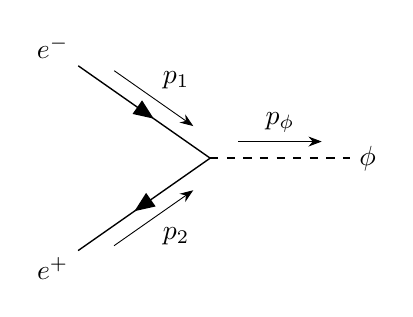
\begin{tikzpicture}
                    \begin{feynhand}
                        \vertex (e1) at (-2, 1.4) {$e^-$};
                        \vertex (e2) at (-2, -1.4) {$e^+$};
                        \vertex (φ) at (2, 0) {$\phi$};
                        \vertex (o) at (0,0);
                        \propag [fermion, momentum = $p_1$] (e1) to (o);
                        \propag [anti fermion, momentum' = $p_2$] (e2) to (o);
                        \propag [scalar, momentum = $p_\phi$] (o) to (φ);
                    \end{feynhand}
                \end{tikzpicture}
            }
            \subcaptionbox{$\phi \to e^- e^+$}{
                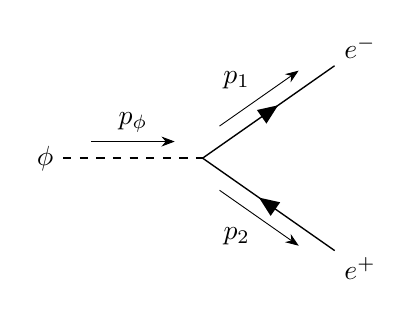
\begin{tikzpicture}
                    \begin{feynhand}
                        \vertex (e1) at (2, 1.4) {$e^-$};
                        \vertex (e2) at (2, -1.4) {$e^+$};
                        \vertex (φ) at (-2, 0) {$\phi$};
                        \vertex (o) at (0,0);
                        \propag [fermion, momentum = $p_1$] (o) to (e1);
                        \propag [anti fermion, momentum' = $p_2$] (o) to (e2);
                        \propag [scalar, momentum = $p_\phi$] (φ) to (o);
                    \end{feynhand}
                \end{tikzpicture}
            }
            \caption{Feynman diagrams for the process $\phi \leftrightarrow e^- e^+$.}
            \label{fig:φee}
        \end{figure}

        The amplitude for the process $\phi \leftrightarrow e^- e^+$ is easy to write down from the corresponding Feynman diagrams in Fig.~\ref{fig:φee}, which is
        \begin{align}
            \ii \mathcal{M}_{\phi \leftarrow e^- e^+} & = \ii y \qty[\bar{v}(p_2) u(p_1)], \\
            \ii \mathcal{M}_{\phi \to e^- e^+} & = \ii y \qty[\bar{u}(p_1) v(p_2)].
        \end{align}
        Therefore, we have \cite{Srednicki:2007qs}
        \begin{align}
            \overline{\sum} \abs{\mathcal{M}_{\phi \leftarrow e^- e^+}}^2 & = y^2 \tr[\qty(-\slashed{p}_1 + m_e) \qty(-\slashed{p}_2 - m_e)] \notag \\
            & = -4 y^2 \qty(p_1 \cdot p_2 + m_e^2), \\
            \overline{\sum} \abs{\mathcal{M}_{\phi \to e^- e^+}}^2 & = y^2 \tr[\qty(-\slashed{p}_1 + m_e) \qty(-\slashed{p}_2 - m_e)] \notag \\
            & = -4 y^2 \qty(p_1 \cdot p_2 + m_e^2).
        \end{align}
        One can see that the squared absolute amplitudes for the process $\phi \leftrightarrow e^- e^+$ are the same, which is consistent with the crossing symmetry.
        Therefore, we have
        \begin{equation}
            \overline{\sum} \abs{\mathcal{M}_{\phi \leftrightarrow e^- e^+}}^2 = -4 y^2 \qty(p_1 \cdot p_2 + m_e^2) = 2 y^2 \qty(m_\phi^2 - 4 m_e^2),
        \end{equation}
        where we have applied the kinematic relation of
        \begin{equation}
            p_1 \cdot p_2 = -\frac{1}{2} m_\phi^2 + m_e^2.
        \end{equation}

        Now we can calculate the collision term for the process $\phi \leftrightarrow e^- e^+$.
        According to Eq.~\eqref{eq:collision-term}, we have
        \begin{equation}
            \begin{aligned}
                C_{\phi \leftrightarrow e^- e^+}[f_\phi] & = && \int \frac{\dd[3]{\vb{p}_1}}{\qty(2 \pi)^3 2 E_1} \frac{\dd[3]{\vb{p}_2}}{\qty(2 \pi)^3 2 E_2} \qty(2 \pi)^4 \delta^{(4)}\qty(p_\phi - p_1 - p_2) \\
                & && {} \times \qty{ \begin{aligned}
                    \qty[1 + f_\phi(\vb{p}_\phi)] f_1(\vb{p}_1) f_2(\vb{p}_2) \overline{\sum} \abs{\mathcal{M}_{\phi \leftarrow e^- e^+}}^2 \\
                    {} - f_\phi(\vb{p}_\phi) \qty[1 - f_1(\vb{p}_1)] \qty[1 - f_2(\vb{p}_2)] \overline{\sum} \abs{\mathcal{M}_{\phi \to e^- e^+}}^2
                \end{aligned} } \\
                & = && 2 y^2 \qty(m_\phi^2 - 4 m_e^2) \int \frac{\dd[3]{\vb{p}_1}}{\qty(2 \pi)^3 2 E_1} \frac{\dd[3]{\vb{p}_2}}{\qty(2 \pi)^3 2 E_2} \qty(2 \pi)^4 \delta^{(4)}\qty(p_\phi - p_1 - p_2) \\
                & && {} \times \qty{f_1(\vb{p}_1) f_2(\vb{p}_2) + f_\phi(\vb{\vb{p}_\phi}) \qty[f_1(\vb{p}_1) + f_2(\vb{p}_2) - 1]}.
            \end{aligned}
        \end{equation}

        According to the assumption that the initial abundance of the scalar boson $\phi$ in the early universe is zero at a sufficiently high temperature, we can simply forbid the scalar boson decay into electron-positron pair, i.e., $f_\phi = 0$ at the sufficiently high temperature.
        This assumption works well if the scalar boson $\phi$ is not in the thermal equilibrium with electrons and positrons. 
        Therefore, we have
        \begin{equation}
            C_{\phi \leftrightarrow e^- e^+}[0] = 2 y^2 \qty(m_\phi^2 - 4 m_e^2) \int \frac{\dd[3]{\vb{p}_1}}{\qty(2 \pi)^3 2 E_1} \frac{\dd[3]{\vb{p}_2}}{\qty(2 \pi)^3 2 E_2} \qty(2 \pi)^4 \delta^{(4)}\qty(p_\phi - p_1 - p_2) f_1(\vb{p}_1) f_2(\vb{p}_2).
            \label{eq:collision-term-φee-0}
        \end{equation}
        Notice that the distribution functions for the electron and positron given by the Fermi-Dirac distribution function as
        \begin{equation}
            f_{1,2} = \frac{1}{\exp(\frac{E - \mu}{T}) + 1}.
        \end{equation}
        However, the chemical potential $\mu_i$'s for the electron and positron are zero since their are relativistic particles at the sufficiently high temperature.
        % Therefore, we have
        % \begin{equation}
        %     f_{1,2} = \frac{1}{\ee^{E/T} + 1}.
        % \end{equation}
        And we usually work in the classical limit, where the distribution functions are given by the Maxwell-Boltzmann distributions as
        \begin{equation}
            f_{1,2} = \ee^{-E / T}.
            \label{eq:Maxwell-Boltzmann-distribution-for-electron-and-positron}
        \end{equation}
        Apply Eq.~\eqref{eq:integration-measure-1-2}, we then have
        \begin{equation}
            \begin{aligned}
                \int \frac{\dd[3]{\vb{p}_\phi}}{(2 \pi)^3 2 E_\phi} C_{\phi \leftrightarrow e^- e^+}[0] & = && \frac{y^2 \qty(m_\phi^2 - 4 m_e^2)}{8 (2 \pi)^3} \int_0^\infty \frac{\dd{\mathrm{p}_\phi^2}}{\sqrt{\mathrm{p}_\phi^2 + m_\phi^2}} \int_{\qty[\mathrm{p}_1^\mathrm{(min)}]^2}^{\qty[\mathrm{p}_1^\mathrm{(max)}]^2} \frac{\dd{\mathrm{p}_1^2}}{\sqrt{\mathrm{p}_1^2 + m_e^2}} \\
                & && {} \times \exp[-\frac{\sqrt{\mathrm{p}_1^2 + m_e^2}}{T}] \exp[-\frac{\sqrt{\mathrm{p}_\phi^2 + m_\phi^2} - \sqrt{\mathrm{p}_1^2 + m_e^2}}{T}]
            \end{aligned}
        \end{equation}

        If we consider the effect of the non-zero $f_\phi$ in the following evolution, the collision term reads
        \begin{equation}
            C_{\phi \leftrightarrow e^- e^+}[f_\phi] = 2 y^2 \qty(m_\phi^2 - 4 m_e^2) \int \frac{\dd[3]{\vb{p}_1}}{\qty(2 \pi)^3 2 E_1} \frac{\dd[3]{\vb{p}_2}}{\qty(2 \pi)^3 2 E_2} \qty(2 \pi)^4 \delta^{(4)}\qty(p_\phi - p_1 - p_2) \qty[f_1 f_2 - f_\phi],
            \label{eq:collision-term-φee-classical-full}
        \end{equation}
        where we do not consider the corrections from the quantum statistics.
        Finally, we show the following evolutions in Fig.~\ref{fig:n_φ-a^3-comparison-of-analytic-and-numeric}.
        The full calculations for these two curves are not shown here.
        We only show the calculations for phase integration measure and some useful integrals in the following sections.

        \begin{figure}
            \begin{tikzpicture}
                \begin{loglogaxis}[
                    xlabel = {$a$},
                    ylabel = {$n_\phi a^3$ [MeV$^{-3}$]},
                    xmin = .9, xmax = 4e6,
                    % xtick = {1, 2, 3, 4, 5, 6, 7, 8, 9, 10},
                    % xticklabel={
                    %     \pgfmathparse{exp(\tick)}%
                    %     \pgfmathprintnumber{\pgfmathresult}
                    % },
                    ymin = 1e-5, ymax = 3e9,
                    % ytick = {1e-10, 1e-9, 1e-8, 1e-7, 1e-6},
                    grid = both,
                    grid style = {solid, gray!30},
                    width = .8\textwidth,
                    height = .5\textwidth,
                    legend style = {at = {(0.5, 0.05)}, anchor = south}
                ]
                    \addplot [mark=none, thick, color=blue] table [x index=0, y index=1,
                    col sep = comma] {data/na3-a-anal-num-comparision.csv};
                    \addlegendentry{analytic result}
                    \addplot [mark=none, thick, color=orange] table [x index=0, y index=2,
                    col sep = comma] {data/na3-a-anal-num-comparision.csv};
                    \addlegendentry{numeric result}
                    % \addlegendentry{$C_{\phi \leftrightarrow e^- e^+}[0]$}      
                \end{loglogaxis}
            \end{tikzpicture}
            \centering
            \caption{
                The comparison of the analytic and numeric results of the total number $n_\phi a^3$ of the scalar boson $\phi$ with the scale factor $a$.
                The analytic result is obtained by joining the production era and the decay era at the turning point $a'$.
            }
            \label{fig:n_φ-a^3-comparison-of-analytic-and-numeric}
        \end{figure}

    \section{Phase Integration Measure}
        In this appendix, we will give the integration measure for the phase space of the particles in the collision term for the 1 $\leftrightarrow$ 2 process.

        \subsection{With Phase Space of \texorpdfstring{$\vb{p}_\phi$}{p\_φ}}
            First, let us consider the integration measure with the phase space of $\vb{p}_\phi$, which reads
            \begin{equation}
                I_3 := \int \frac{\dd[3]{\vb{p}_\phi}}{\qty(2 \pi)^3 2 E_\phi} \frac{\dd[3]{\vb{p}_1}}{\qty(2 \pi)^3 2 E_1} \frac{\dd[3]{\vb{p}_2}}{\qty(2 \pi)^3 2 E_2} \qty(2 \pi)^4 \delta^{(4)}\qty(p_\phi - p_1 - p_2),
            \end{equation}
            where $m_1 = m_2 = m_e$ and $E_i = \sqrt{\vb{p}_i^2 + m_e^2}$.

            According to the symmetry of SO(3) rotation of $\vb{p}_\phi$, we have
            \begin{equation}
                I_3 = \frac{4 \pi}{(2 \pi)^3} \int_0^\infty \frac{\mathrm{p}_\phi^2 \dd{\mathrm{p}_\phi}}{2 E_\phi} \int \frac{\dd[3]{\vb{p}_1}}{\qty(2 \pi)^3 2 E_1} \frac{\dd[3]{\vb{p}_2}}{\qty(2 \pi)^3 2 E_2} \qty(2 \pi)^4 \delta^{(4)}\qty(p_\phi - p_1 - p_2),
            \end{equation}
            where $\mathrm{p}_i := \abs{\vb{p}_i}$.
            Without loss of generality, we can choose the $z$-axis as the direction of $\vb{p}_\phi$, i.e., $p_\phi^\mu = \qty(E_\phi, 0, 0, \mathrm{p}_\phi)$.
            The integration over $\vb{p}_2$ with the three-dimensional delta function gives trivially
            \begin{equation}
                \int \frac{\dd[3]{\vb{p}_2}}{\qty(2 \pi)^3 2 E_2} \qty(2 \pi)^4 \delta^{(4)}\qty(p_\phi - p_1 - p_2) = \frac{2 \pi}{2 E_2} \delta(E_\phi - E_1 - E_2).
            \end{equation}
            Now we can consider the parametrization of $\vb{p}_1$ as $\vb{p}_1 = \qty(\mathrm{p}_1 \sin \theta \sin \varphi, \mathrm{p}_1 \sin \theta \cos \varphi, \mathrm{p}_1 \cos\theta)$, which simplifies the integration over $\vb{p}_1$ as
            \begin{equation}
                \begin{aligned}
                    \int \frac{\dd[3]{\vb{p}_1}}{\qty(2 \pi)^3 2 E_1} & = \frac{1}{(2 \pi)^3} \int_0^\infty \frac{\mathrm{p}_1^2 \dd{\mathrm{p}_1}}{2 E_1} \int_{-1}^{+1} \dd{\cos \theta} \int_0^{2 \pi} \dd{\varphi} \\
                    & = \frac{1}{(2 \pi)^2} \int_0^\infty \frac{\mathrm{p}_1^2 \dd{\mathrm{p}_1}}{2 E_1} \int_{-1}^{+1} \dd{\cos \theta}.
                \end{aligned}
            \end{equation}
            Therefore, the total integration reads
            \begin{equation}
                I_3 = \frac{4 \pi}{(2 \pi)^4} \int_0^\infty \frac{\mathrm{p}_\phi^2 \dd{\mathrm{p}_\phi}}{2 E_\phi} \int_0^\infty \frac{\mathrm{p}_1^2 \dd{\mathrm{p}_1}}{2 E_1} \int_{-1}^{+1} \dd{\cos \theta} \frac{\delta(E_\phi - E_1 - E_2)}{2 E_2}.
            \end{equation}

            For the integration of
            \begin{equation}
                \int_{-1}^{+1} \dd{\cos \theta} \delta(E_\phi - E_1 - E_2) = \int_{-1}^{+1} \dd{q} \delta\qty(E_\phi - E_1 - \sqrt{\mathrm{p}_\phi^2 + \mathrm{p}_1^2 + m_e^2 - 2 \mathrm{p}_\phi \mathrm{p}_1 q}),
            \end{equation}
            we can use the formula of the delta function as
            \begin{equation}
                \int \dd{x} \delta(f(x)) = \sum_i \frac{1}{\abs{f'(x_i)}},
            \end{equation}
            where $x_i$ are the roots of $f(x) = 0$.
            Then we have
            \begin{equation}
                \int_{-1}^{+1} \dd{q} \delta\qty(E_\phi - E_1 - \sqrt{\mathrm{p}_\phi^2 + \mathrm{p}_1^2 + m_e^2 - 2 \mathrm{p}_\phi \mathrm{p}_1 q}) = \frac{E_2}{\mathrm{p}_\phi \mathrm{p}_1}
            \end{equation}
            if
            \begin{equation}
                \sqrt{\mathrm{p}_\phi^2 + \mathrm{p}_1^2 + m_e^2 - 2 \mathrm{p}_\phi \mathrm{p}_1} \le E_\phi - E_1 \le \sqrt{\mathrm{p}_\phi^2 + \mathrm{p}_1^2 + m_e^2 + 2 \mathrm{p}_\phi \mathrm{p}_1}.
            \end{equation}
            Else, the integral is zero.
            The condition for this integral to be non-zero will give the restriction on the integration interval of $\mathrm{p}_1$, which reads
            \begin{equation}
                \frac{1}{2} \abs{\mathrm{p}_\phi - \sqrt{\frac{\qty(m_\phi^2 - 4 m_e^2) \qty(m_\phi^2 + \mathrm{p}_\phi^2)}{m_\phi^2}}} \le p_1 \le \frac{1}{2} \qty[\mathrm{p}_\phi + \sqrt{\frac{\qty(m_\phi^2 - 4 m_e^2) \qty(m_\phi^2 + \mathrm{p}_\phi^2)}{m_\phi^2}}].
                \label{eq:bounds-of-q1}
            \end{equation}

            Therefore, the integration measure is finally given by
            \begin{equation}
                \begin{aligned}
                    I_3 & = \frac{1}{(2 \pi)^3} \int_0^\infty \frac{\mathrm{p}_\phi \dd{\mathrm{p}_\phi}}{2 E_\phi} \int_{\mathrm{p}_1^\mathrm{(min)}}^{\mathrm{p}_1^\mathrm{(max)}} \frac{\mathrm{p}_1 \dd{\mathrm{p}_1}}{2 E_1} \\
                    & = \frac{1}{16 (2 \pi)^3} \int_0^\infty \frac{\dd{\mathrm{p}_\phi^2}}{\sqrt{\mathrm{p}_\phi^2 + m_\phi^2}} \int_{\qty[\mathrm{p}_1^\mathrm{(min)}]^2}^{\qty[\mathrm{p}_1^\mathrm{(max)}]^2} \frac{\dd{\mathrm{p}_1^2}}{\sqrt{\mathrm{p}_1^2 + m_e^2}},
                \end{aligned}
                \label{eq:integration-measure-1-2}
            \end{equation}
            where $\mathrm{p}_1^\mathrm{(min)}$ and $\mathrm{p}_1^\mathrm{(max)}$ are the lower and upper bounds of the integration interval of $\mathrm{p}_1$ given in Eq.~\eqref{eq:bounds-of-q1}, respectively.
        
        \subsection{Without Phase Space of \texorpdfstring{$\vb{p}_\phi$}{p\_φ}}
            If we do not consider the phase space of $\vb{p}_\phi$, the integration measure is given by
            \begin{equation}
                \tilde{I}_2(p_\phi) := \int \frac{\dd[3]{\vb{p}_1}}{\qty(2 \pi)^3 2 E_1} \frac{\dd[3]{\vb{p}_2}}{\qty(2 \pi)^3 2 E_2} \qty(2 \pi)^4 \delta^{(4)}\qty(p_\phi - p_1 - p_2).
            \end{equation}
            Following the same procedure as the case with the phase space of $\vb{p}_\phi$, we have
            \begin{equation}
                \begin{aligned}
                    \tilde{I}_2(p_\phi) & = \frac{1}{2 \pi} \int_0^\infty \frac{\mathrm{p}_1^2 \dd{\mathrm{p}_1}}{2 E_1} \int_{-1}^{+1} \dd{\cos \theta} \frac{\delta(E_\phi - E_1 - E_2)}{2 E_2} \\
                    & = \frac{1}{8 \pi \mathrm{p}_\phi} \int_{\mathrm{p}_1^\mathrm{(min)}}^{\mathrm{p}_1^\mathrm{(max)}} \frac{\mathrm{p}_1 \dd{\mathrm{p}_1}}{E_1} \\
                    & = \frac{1}{8 \pi \mathrm{p}_\phi} \int_{\qty[\mathrm{p}_1^\mathrm{(min)}]^2}^{\qty[\mathrm{p}_1^\mathrm{(max)}]^2} \frac{\dd{\mathrm{p}_1^2}}{\sqrt{\mathrm{p}_1^2 + m_e^2}},
                \end{aligned}
            \end{equation}
            where the bounds of the integration interval of $\mathrm{p}_1$ are the same as Eq.~\eqref{eq:bounds-of-q1}.

        \section{Useful Integrals}
            In this appendix, we will give some useful integrals for the calculation of the collision term.

            In the calculation of the collision term, we need to calculate the following integral of
            \begin{equation}
                F_1(m, T) := \int_0^\infty \frac{p^2 \dd{p}}{\sqrt{p^2 + m^2}} \exp[-\frac{\sqrt{p^2 + m^2}}{T}],
                \label{eq:F_1-definition}
            \end{equation}
            where $m \ge 0$ and $T > 0$.
            If $m = 0$, the integral is trivially given by
            \begin{equation}
                F_1(0, T) = \int_0^\infty p \exp[-\frac{p}{T}] \dd{p} = T^2.
                \label{eq:F_1-evaluation-m=0}
            \end{equation}
            If $m > 0$, we can use the substitution of $p = m \sinh x$ to simplify the integral as
            \begin{equation}
                F_1(m, T) = m^2 \int_0^\infty \sinh^2 x \exp[-\frac{m \cosh x}{T}] \dd{x},
            \end{equation}
            which could be futher converted to the integral representation of the modified Bessel function of the second kind as \cite[Eq.~(\href{https://dlmf.nist.gov/10.32.8}{10.32.8})]{NIST:DLMF}
            \begin{equation}
                K_\nu(z) \equiv \frac{\sqrt{\pi}}{\Gamma\qty(\nu + \frac{1}{2})} \qty(\frac{z}{2})^\nu \int_0^\infty \ee^{-z \cosh t} \sinh^{2 \nu} t \dd{t}
            \end{equation}
            with $\Re \nu > -1 / 2$ and $\abs{\arg z} < \pi / 2$.
            Therefore, we have $\nu = 1$ and $z = m / T$, which lead to
            \begin{equation}
                F_1(m, T) = m T K_1\qty(\frac{m}{T}).
                \label{eq:F_1-evaluation}
            \end{equation}
            
            The second integral we need to calculate is given by
            \begin{equation}
                F_2(m, T) := \int_0^\infty p^2 \exp[-\frac{\sqrt{p^2 + m^2}}{T}] \dd{p},
                \label{eq:F_2-definition}
            \end{equation}
            where $m \ge 0$ and $T > 0$, too.
            If $m = 0$, the integral is trivially given by
            \begin{equation}
                F_2(0, T) = \int_0^\infty p^2 \exp[-\frac{p}{T}] \dd{p} = 2 T^3.
                \label{eq:F_2-evaluation-m=0}
            \end{equation}
            If $m > 0$, we can also use the substitution of $p = m \sinh x$ to simplify the integral as
            \begin{equation}
                \begin{aligned}
                    F_2(m, T) & = m^3 \int_0^\infty \exp[-\frac{m \cosh x}{T}] \sinh^2 x \cosh x \dd{x} \\
                    & = \frac{m^3}{4} \int_0^\infty \exp[-\frac{m \cosh x}{T}] \qty(\cosh 3 x - \cosh x) \dd{x} \\
                \end{aligned},
            \end{equation}
            which could be also converted to the integral representation of the modified Bessel function of the second kind as \cite[Eq.~(\href{https://dlmf.nist.gov/10.32.9}{10.32.9})]{NIST:DLMF}
            \begin{equation}
                K_\nu(z) \equiv \int_0^\infty \ee^{-z \cosh t} \cosh(\nu t) \dd{t}
            \end{equation}
            with $\abs{\arg z} < \pi / 2$.
            Therefore, we have $\nu = 1, 3$ and $z = m / T$, which lead to
            \begin{equation}
                \begin{aligned}
                    F_2(m, T) & = \frac{m^3}{4} \qty[K_3\qty(\frac{m}{T}) - K_1\qty(\frac{m}{T})] \\
                    & = m^2 T K_2\qty(\frac{m}{T}).
                \end{aligned}
                \label{eq:F_2-evaluation}
            \end{equation}
            The last step is simplified via \textsc{Wolfram Mathematica}.

            The third integral we are interested in is given by
            \begin{equation}
                F_3(a, m) := \int_{a}^\infty t^3 K_1(m t) \dd{t},
                \label{eq:F_3-definition}
            \end{equation}
            where $a \ge 0$ and $m > 0$.
            With the substitution of $m t = x$, we have
            \begin{equation}
                F_3(a, m) = \frac{1}{m^4} \int_{m a}^\infty x^3 K_1(x) \dd{x}.
            \end{equation}
            If $a = 0$, the integral is trivially given by \cite[Eq.~(\href{https://dlmf.nist.gov/10.43.19}{10.43.19})]{NIST:DLMF}
            \begin{equation}
                \begin{aligned}
                    F_3(0, m) & = \frac{1}{m^4} \int_0^\infty x^3 K_1(x) \dd{x} \\
                    & = \frac{4}{m^4} \Gamma\qty(2 - \frac{1}{2}) \Gamma\qty(2 + \frac{1}{2}) \\
                    & = \frac{3 \pi}{2 m^4}.
                \end{aligned}
            \end{equation}
            If $a > 0$, we can have
            \begin{equation}
                \begin{aligned}
                    F_3(a, m) & = F_3(0, m) - \frac{1}{m^4} \int_0^{m a} x^3 K_1(x) \dd{x} \\
                    & = \frac{3 \pi}{2 m^4} - \frac{1}{m^4} \int_0^{m a} x^3 K_1(x) \dd{x}.
                \end{aligned}
            \end{equation}
            From \textsc{Wolfram Mathematica}, we have
            \begin{equation}
                \int_0^t x^3 K_1(x) \dd{x} = 4 G^{2,1}_{1,3}\qty(\frac{t^2}{4} \middle| \begin{array}{c} 1 \\ \frac{3}{2}, \frac{5}{2}, 0 \end{array} )
            \end{equation}
            with $t > 0$, where $G^{m,n}_{p,q}$ is the Meijer $G$ function.
            Therefore, we have
            \begin{equation}
                F_3(a, m) = \frac{3 \pi}{2 m^4} - \frac{4}{m^4} G^{2,1}_{1,3}\qty(\frac{m^2 a^2}{4} \middle| \begin{array}{c} 1 \\ \frac{3}{2}, \frac{5}{2}, 0 \end{array} ).
                \label{eq:F_3-evaluation}
            \end{equation}

    \printbibliography[heading=bibintoc]
\end{document}
